
\section{Asymmetric Cryptography}

\paragraph{Public Key Encryption (PKE) Scheme}
is a triple $PKE = (KGen, Enc, Dec)$.
\\
$KGen$ generates a key pair $(sk, pk) \in \mathcal{SK} \times \mathcal{PK}$. \\
$Enc$ takes a public key $pk$ and a message $m \in \M \subseteq \setzeroone^*$
and produces a ciphertext $c \in \C \subseteq \setzeroone^*$. \\
$Dec$ takes a private key $sk$ and a ciphertext and produces a message or an error $\bot$.
\\
For correctness, we require that $Dec_{sk}( Enc_{pk}(m) ) = m$ (for all keypairs output by $KGen$).

\paragraph{Key distribution}
PKE translates the problem of securely distributing secret symmetric keys into
distributing authentic public keys.

\paragraph{IND-CCA Security}
The adversary gets access to a LoR encryption and a decryption oracle and needs to
distinguish whether the left or the right messages are being encrypted
(see \autoref{fig:pke-ind-cca}).
Compare this with the symmetric game (given in \autoref{fig:ind-cca}).
\\
IND-CPA security is defined the same, but without the decryption oracle.

\begin{figure}[h]
    \centering
	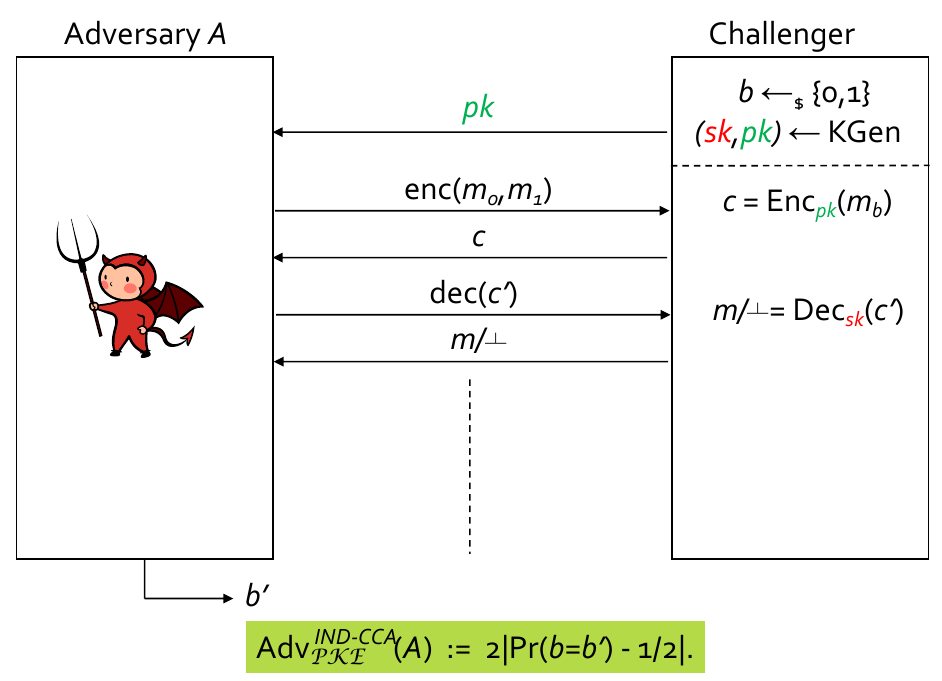
\includegraphics[scale=0.4]{images/pke-ind-cca.png}
    \caption{IND-CCA game for PKE}
    \label{fig:pke-ind-cca}
\end{figure}

\paragraph{Integrity for PKE}
Defining integrity does not make sense in a PKE setting.
Anybody can choose a message, encrypt it under the public key and can thus come
up with a valid ciphertext that will be accepted by the receiver.


\subsection{KEM/DEM Paradigm}

\paragraph{Hybrid encryption}
Asymmetric crypto is expensive (e.g. due to large key sizes).
Idea: encrypt the message symmetrically and encrypt the symmetric key using PKE.

\paragraph{Key Encapsulation Mechanism KEM}
is a triple $(KGen, Encap, Decap)$.
\\
$KGen$ generates a random key pair $(sk, pk)$. \\
$Encap$ takes a public key $pk$ and generates a random key $K$, outputting the encapsulation $c$ and the generated key: $(c, K) \in \C \times \K$. \\
$Decap$ takes a private key $sk$ and an encapsulation $c$ and outputs either the key $K$ or an error $\bot$.
\\
For correctness, we require that if $(c, K) \leftarrow Encap(pk)$ then $K \leftarrow Decap(sk, c)$.

Note that unlike PKE, $Encap$ has no message input.
Instead, it internally generates a key.

\paragraph{IND-CCA Security for KEMs}
The adversary needs to distinguish between an encapsulated key $K_0$
(for which it gets the encapsulation $c$) and a randomly generated key $K_1$.
See \autoref{fig:kem-ind-cca}.

\begin{figure}[h]
    \centering
	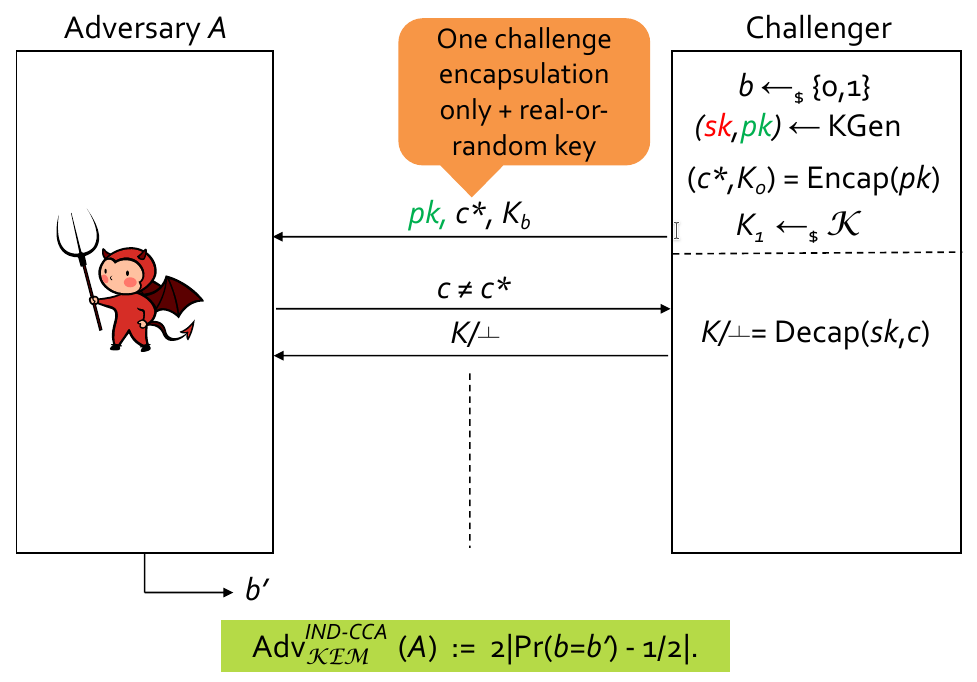
\includegraphics[scale=0.4]{images/kem-ind-cca.png}
    \caption{IND-CCA game for KEM}
    \label{fig:kem-ind-cca}
\end{figure}

\paragraph{Data Encapsulation Mechanism DEM}
is simply a symmetric encryption scheme.

\paragraph{KEM/DEM Composition Paradigm}
We can build a PKE scheme from a KEM and a DEM:
\\
$PKE.KGen$:
$(sk, pk) = KEM.KGen()$; return $(sk, pk)$
\\
$PKE.Enc$:
$(c_0, K) = KEM.Encap(pk)$; $c_1 = DEM.Enc(K, m)$; return $(c_0, c_1)$
\\
$PKE.Dec$:
$m = \bot$; $K = KEM.Decap(sk, c_0)$; if $K \neq \bot$ then $m = DEM.Dec(K, c_1)$; return $m$

Theorem: If both KEM and DEM are IND-CCA secure, then so is the composed PKE.
The proof proceeds using game hopping.


\subsection{RSA}

\paragraph{Textbook RSA}\mbox{}\\
$KGen$:
Generates random primes $p, q$ of size $\frac{k}{2}$ bits.
Sets $N=pq$.
Also generates integers $d, e$ such that $de = 1 \mod (p-1)(q-1)$.
Outputs keypair $(sk, pk)$ s.t. $sk = d$ and $pk = (e, N)$.
\\
$Enc$:
Outputs $c = m^e \mod N$.
\\
$Dec$:
Outputs $m = c^d \mod N$.

\textbf{NOT secure}.
Not randomised, so cannot satisfy IND-CPA.
Also malleable: $(m_0 \cdot m_1)^e = m_0^e \cdot m_1^e $.

Questions:
How to generate $p, q, d, e$?
How to encode messages as integers in $[1, N-1]$?

\paragraph{Generating keys}
Needs a good source of randomness and primality test.
Things can still go wrong:
shared prime factors\footnote{See ``Mining your p's and q's.''},
over-optimised prime generation, bad primality tests.

From $e$, $d$ can be calculated using the Extended Euclidean algorithm (knowing $p, q$).
In practice, $e = 2^{16}+1 = 65537$ is often used for faster encryption (prime + likely coprime to $(p-1)(q-1)$).

Other optimisations lead to vulnerabilities:
\begin{itemize}
\item Small $e$:
If $e$ is small (e.g. $e=3$), then for small messages it can happen that $c=m^3$ holds over the integers, i.e. without modular reduction.
Then an attacker can simply take the (cube) root to recover $m$.
\item Small $d$:
insecure up for $d \leq N^{1/4}$ (Weiner's attack)
\end{itemize}

\paragraph{Keysize requirements}
By breaking the \emph{Integer Factorisation Problem (IFP)} (to factor $N$) we can break RSA (the reverse may not hold!).
One algorithm for the IFP is the \emph{Number Field Sieve (NFS)}.
Generally, the best known algorithms are super-polynomial, but sub-exponential.

See \href{https://www.keylength.com/}{keylength.com} for key size recommendations.

\paragraph{Malleability}
Since textbook RSA is malleable, an attacker can choose an arbitrary $s$ and amend the message:
$s^e \cdot c \mod N$ decrypts to $s \cdot m \mod N$.

\paragraph{Padding}
Goals:
introduce randomness,
expand short messages to full size,
and destroy algebraic relationship (removing malleability property)
to achieve IND-CCA security.

\paragraph{PKCS\#1 v1.5 Padding}
Structure:
Two most significant bytes set to \mbox{\texttt{0x00 0x02}},
then $\geq 8$ random non-zero bytes,
then a zero byte and finally the message $m$ as the left most bytes.
Implies a maximum message size of $k-11$ bytes (assuming $N$ as $k$ bytes).

Encryption: $pad(m)^e \mod N$ \\
Decryption: $m' = c^d \mod N$, then check for correct padding and return $m$.

\underline{Not} IND-CCA secure.

\begin{figure}[h]
    \centering
	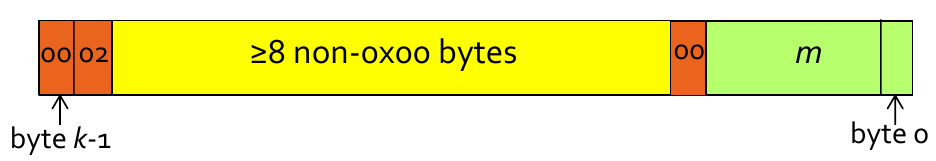
\includegraphics[scale=0.4]{images/rsa-pkcs.png}
    \caption{PKCS\#1 v1.5 Padding}
    \label{fig:rsa-pkcs}
\end{figure}

\paragraph{Bleichenbacher's Attack on PKCS\#1 v1.5}
Let $m' = (00\ 02\ ||\ r\ ||\ 00\ ||\ m)$ be the encoded message and let $c = m'^e \mod N$.
Attacker asks oracle to decrypt $s^e \cdot c \mod N$.
With probability $\approx 2^{-16}$ the padding is valid and decryption does not return a padding error.
\\
Through an \emph{adaptive attack}, using carefully chosen $s$, one can eventually recover $m'$ (and thus $m$).

Originally this required around $2^{20}$ queries but has since improved to 5-10K queries for a 1024 bit modulus.
For attacks against TLS, see \href{https://drownattack.com/}{DROWN} and \href{https://robotattack.org/}{ROBOT}.

\paragraph{RSA-OAEP Padding}
Optimal Asymmetric Encryption Padding, standardised in PKCS\#1 v2.1, yet not as widely adopted.

Setup:
Let $n$ be the bitsize of $N$.
Let $k_0, k_1$ be such that no adversary can perform neither $2^{k_0}$ nor $2^{k_1}$ operations in reasonable time (e.g. 128).
Messages are assumed to be bitstrings of length $n - k_0 - k_1$.
Let $G, H$ be hash functions such that
$G: \setzeroone^{k_0} \mapsto \setzeroone^{n-k_0}$
and $H: \setzeroone^{n-k_0} \mapsto \setzeroone^{k_0}$.

Encoding:
See \autoref{fig:rsa-oaep}.
At the end, compute $c = (X\ ||\ Y)^e \mod N$.

Decoding:
decrypt, then reverse the encoding, then check for the presence of the zero bits.

Can be proven to be IND-CCA secure (under strong number theoretic assumptions, including the Random Oracle Model).
Intuition: output of hash functions is random, breaking up any algebraic relationships.

\begin{figure}[h]
    \centering
	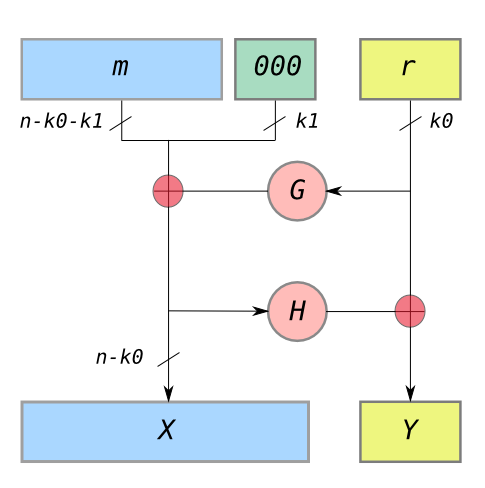
\includegraphics[scale=0.45]{images/rsa-oaep.png}
    \caption{RSA-OAEP Padding}
    \label{fig:rsa-oaep}
\end{figure}

\paragraph{Random Oracle Model ROM}
Strong abstraction of hash functions: models hash functions as truly random functions.

A practical problem for proofs is that evaluating a random function can take exponential time -- but we only consider poly-time adversaries!
We solve this by ``stopping time'' when the adversary invokes a hash function,
and forcing the adversary to use an oracle to evaluate the hash function for them.
This extra oracle can inspect the adversary's queries, sample new random values for fresh queries, and return the values for repeated queries from its cache.

\paragraph{RSA (Inversion) Problem}
Summarizes the task of performing an RSA private-key operation given only the public key.
Specifically for decryption, the task is to compute $m$ given only $c$ and $(e, N)$.

One -- but not the only -- way to solve this is by factoring $N$.
There is no proof that the IFP or the RSA problem are (computationally) hard.
The RSA problem is at least as easy as the IFP, but it might be easier.
(Finding $d$ is equivalent to factoring though.)


\subsection{Diffie-Hellman Key Exchange}


\subsection{Elgamal}
 
